\chapter{Mekanika Lagrange}\label{ch:b3:lagrangian-mechanics}

Cobalah menuliskan hukum Newton untuk sebuah bandul ganda: dua gaya
tegangan, tak satu pun diketahui lebih dahulu, keduanya berubah arah
setiap saat, dan empat persamaan skalar yang harus diurai hanya untuk
mengetahui bagaimana dua sudut berkembang. Lakukanlah hal yang sama
untuk manik pada gelang yang berputar, untaian pegas terkopel, atau
lengan robot. Gaya yang menahan sebuah sistem tetap utuh --- batang,
rel, engsel --- tidak melakukan usaha sedikit pun, namun cara Newton
memaksa kita membawanya dalam setiap perhitungan. Bab ini menyajikan
perumusan ulang yang diterbitkan Lagrange pada 1788: gambarkanlah
sistemnya dengan sedikit koordinat yang memang dapat berubah,
tuliskanlah satu fungsi tunggal $L = E_k - E_p$, dan satu resep
menghasilkan persamaan geraknya dalam koordinat apa pun, dengan setiap
batang dan rel sudah tersingkir lebih dahulu. Lebih dari itu, perumusan
baru ini menampakkan apa yang disembunyikan perumusan Newton: setiap
simetri $L$ melahirkan satu besaran kekal --- momentum dari keseragaman
ruang, energi dari keseragaman waktu --- hasil karya Emmy Noether yang
kini menjadi asas penata fisika jauh melampaui mekanika.

\section{Dari gaya ke koordinat}

\begin{definition}[Kendala, derajat kebebasan, koordinat rampatan]\label{def:b3:lagrangian-mechanics:coordinates}
\index{kendala}\index{derajat kebebasan}\index{koordinat rampatan}
Yang disebut \emph{kendala} adalah syarat geometris yang dikenakan pada
kedudukan sebuah sistem --- manik tetap berada pada kawatnya, batang
sebuah bandul mempertahankan panjang tetap, dua roda pada satu as
berputar bersama. Kendala yang dapat dinyatakan sebagai persamaan
$f(\vect r_1, \dots, \vect r_N, t) = 0$ di antara koordinatnya (dan
mungkin juga waktu) disebut \emph{holonomik}. Banyaknya cara bebas yang
masih tersisa bagi konfigurasinya untuk berubah adalah jumlah
\emph{derajat kebebasan} $n$; setiap himpunan $n$ besaran bebas
$q_1, \dots, q_n$ yang menetapkan konfigurasinya secara lengkap
merupakan satu himpunan \emph{koordinat rampatan} --- sudut, panjang,
atau campuran keduanya sesuka kita. Turunan waktunya
$\dot q_1, \dots, \dot q_n$ adalah
\emph{kecepatan rampatan}\index{kecepatan rampatan}.
\end{definition}

\begin{example}[Menghitung derajat kebebasan]\label{ex:b3:lagrangian-mechanics:counting}
Sebuah titik pada meja: $n = 2$. Bandul bidang berpanjang tetap: satu
sudut, $n = 1$. Bandul ganda: dua sudut, $n = 1 + 1 = 2$. Manik pada
gelang tegar: satu sudut, $n = 1$ --- sekalipun gelangnya sendiri
dipaksa berputar, karena putaran yang dikenakan itu tidak menambah
kebebasan. Benda tegar yang bebas di ruang: tiga koordinat pusatnya
ditambah tiga sudut, $n = 6$. Gas berisi $N$ molekul bebas (titik):
$n = 3N$. Setiap \omterm{def:b3:lagrangian-mechanics:coordinates}{kendala} holonomik menghapus satu \omterm{def:b3:lagrangian-mechanics:coordinates}{derajat kebebasan}:
dua titik yang dihubungkan sebuah batang mempunyai $3 + 3 - 1 = 5$.
\end{example}

\begin{omfigure}
\begin{tikzpicture}[font=\small, >=Stealth]
  % (a) plane pendulum
  \begin{scope}
    \draw[thick] (-1,0) -- (1,0);
    \foreach \i in {-0.8,-0.5,-0.2,0.1,0.4,0.7} \draw (\i,0) -- (\i+0.18,0.16);
    \fill (0,0) circle (1.5pt);
    \draw[dashed] (0,0) -- (0,-2.2);
    \draw[thick] (0,0) -- (-55:2.1);
    \fill[omDef] (-55:2.1) circle (3pt);
    \draw[->] (0,-1.0) arc (-90:-55:1.0);
    \node at (-72:1.35) {$\theta$};
    \node at (-55:2.5) {$m$};
    \node at ($(-55:1.35)+(0.28,0.12)$) {$\ell$};
    \node at (0,-2.9) {satu koordinat: $\theta$};
  \end{scope}
  % (b) bead on rotating hoop
  \begin{scope}[xshift=6.2cm]
    \coordinate (C) at (0,-2.35);
    \draw[thick] (C) circle (1.55);
    \draw[dashed] (0,-0.3) -- (0,-4.6);
    \draw[->, thick] (0.35,-0.15) arc (20:160:0.37);
    \node at (0,0.25) {$\omega$};
    \fill (C) circle (1pt);
    \draw (C) -- ++(-50:1.55);
    \fill[omDef] ($(C)+(-50:1.55)$) circle (3pt);
    \draw[->] ($(C)+(0,-0.85)$) arc (-90:-50:0.85);
    \node at ($(C)+(-70:1.18)$) {$\theta$};
    \node at ($(C)+(-38:2.0)$) {$m$};
    \draw (C) -- ++(135:1.55);
    \node at (-1.35,-1.35) {$R$};
    \node at (0,-4.95) {satu koordinat: $\theta$};
  \end{scope}
  % (c) double pendulum
  \begin{scope}[xshift=11.4cm]
    \draw[thick] (-0.9,0) -- (0.9,0);
    \foreach \i in {-0.7,-0.4,-0.1,0.2,0.5} \draw (\i,0) -- (\i+0.18,0.16);
    \fill (0,0) circle (1.5pt);
    \draw[dashed] (0,0) -- (0,-1.7);
    \draw[thick] (0,0) -- (-65:1.5) coordinate (m1);
    \fill[omDef] (m1) circle (2.6pt);
    \draw[dashed] (m1) -- ++(0,-1.5);
    \draw[thick] (m1) -- ++(-40:1.5) coordinate (m2);
    \fill[omThm] (m2) circle (2.6pt);
    \draw[->] (0,-0.8) arc (-90:-65:0.8);
    \node at (-80:1.1) {$\theta_1$};
    \draw[->] ($(m1)+(0,-0.75)$) arc (-90:-40:0.75);
    \node at ($(m1)+(-68:1.05)$) {$\theta_2$};
    \node at (0.3,-3.4) {dua koordinat: $\theta_1, \theta_2$};
  \end{scope}
\end{tikzpicture}

{\small \omterm{def:b3:lagrangian-mechanics:coordinates}{Koordinat rampatan}: setiap sistem digambarkan oleh sudut yang
memang dapat berubah, bukan oleh koordinat Kartesius massanya. Tegangan
batang dan gaya normal gelangnya tak pernah muncul.}
\end{omfigure}

\section{Asas aksi terkecil}

\begin{definition}[Lagrangian dan aksi]\label{def:b3:lagrangian-mechanics:action}
\index{Lagrangian}\index{aksi}
Yang disebut \emph{Lagrangian} sebuah sistem mekanis yang gayanya
diturunkan dari energi potensial $E_p$ adalah fungsi koordinat,
kecepatan, dan mungkin juga waktu
\[
L(q, \dot q, t) = E_k - E_p ,
\]
yaitu energi kinetik \emph{dikurangi} energi potensial, keduanya
dinyatakan dalam \omterm{def:b3:lagrangian-mechanics:coordinates}{koordinat rampatan}. Yang disebut \emph{aksi} sebuah
gerak terbayangkan $q(t)$ antara dua ujung tetap $q(t_1)$ dan $q(t_2)$
adalah bilangan
\[
S[q] = \int_{t_1}^{t_2} L\big(q(t), \dot q(t), t\big)\,\dd t .
\]
$S$ adalah sebuah \emph{fungsional}: ia melahap seluruh lintasan dan
mengembalikan satu bilangan, dalam joule-sekon --- satuan tetapan Planck.
\end{definition}

\begin{theorem}[Asas Hamilton dan persamaan Euler--Lagrange]\label{thm:b3:lagrangian-mechanics:euler-lagrange}
\index{asas Hamilton}\index{persamaan Euler--Lagrange}\index{aksi terkecil}
Di antara semua gerak terbayangkan yang menghubungkan dua ujung yang
sama dalam selang waktu yang sama, gerak yang sesungguhnya adalah gerak
yang membuat \omterm{def:b3:lagrangian-mechanics:action}{aksinya} \emph{stasioner} (\emph{asas Hamilton}, atau asas
\emph{\omterm{thm:b3:lagrangian-mechanics:euler-lagrange}{aksi terkecil}}). Setara dengan itu, geraknya memenuhi
\emph{\omterm{thm:b3:lagrangian-mechanics:euler-lagrange}{persamaan Euler--Lagrange}}
\[
\frac{\dd}{\dd t}\frac{\partial L}{\partial\dot q_i}
 - \frac{\partial L}{\partial q_i} = 0 ,
\qquad i = 1, \dots, n :
\]
satu persamaan orde dua untuk tiap \omterm{def:b3:lagrangian-mechanics:coordinates}{derajat kebebasan}, dalam koordinat
apa pun yang dipilih.
\end{theorem}

\begin{proof}
Ubahlah bentuk lintasannya: $q_i(t) \to q_i(t) + \delta q_i(t)$ dengan
$\delta q_i(t_1) = \delta q_i(t_2) = 0$. Sampai orde pertama,
\[
\delta S = \int_{t_1}^{t_2}\sum_i\Big(
  \frac{\partial L}{\partial q_i}\,\delta q_i
 + \frac{\partial L}{\partial\dot q_i}\,\delta\dot q_i\Big)\dd t
 = \int_{t_1}^{t_2}\sum_i\Big(
  \frac{\partial L}{\partial q_i}
 - \frac{\dd}{\dd t}\frac{\partial L}{\partial\dot q_i}\Big)\delta q_i\,\dd t ,
\]
setelah suku keduanya diintegralkan parsial ($\delta\dot q_i =
\dd(\delta q_i)/\dd t$) dan suku batasnya dibuang, karena suku itu
lenyap di kedua ujung yang tetap. Jika $\delta S = 0$ untuk
\emph{setiap} perubahan bentuk, kurungnya harus lenyap pada setiap saat
dan untuk tiap $i$ --- seandainya ia positif di suatu tempat, sebuah
tonjolan $\delta q_i$ yang terpusat di sana akan memberi
$\delta S \neq 0$. Kebalikannya terbaca pada baris yang sama.
\end{proof}

\begin{omfigure}
\begin{tikzpicture}[font=\small, >=Stealth]
  \draw[->] (0,0) -- (7.6,0) node[right] {$t$};
  \draw[->] (0,0) -- (0,3.4) node[above] {$q$};
  \fill (0.8,0.7) circle (2pt) node[below left] {$q(t_1)$};
  \fill (6.8,2.3) circle (2pt) node[above right] {$q(t_2)$};
  \draw[omDef, very thick] (0.8,0.7) .. controls (2.6,2.6) and (5.0,1.4) .. (6.8,2.3);
  \draw[omExo, dashed] (0.8,0.7) .. controls (2.2,0.6) and (5.4,0.9) .. (6.8,2.3);
  \draw[omExo, dashed] (0.8,0.7) .. controls (3.0,3.6) and (5.2,2.9) .. (6.8,2.3);
  \node[omDef] at (1.9,3.35) {lintasan sesungguhnya};
  \draw[->, omDef] (2.25,3.15) -- (2.85,2.3);
  \node[omExo] at (3.4,0.42) {lintasan variasi};
  \draw[<->] (4.1,1.62) -- (4.1,2.62);
  \node at (4.55,2.15) {$\delta q$};
\end{tikzpicture}

{\small Asas Hamilton: di antara semua lintasan berujung dan berdurasi
sama, lintasan yang sesungguhnya membuat $S = \int L\,\dd t$ stasioner
--- perubahan bentuk $\delta q$ orde pertama mengubah $S$ hanya pada
orde kedua.}
\end{omfigure}

\begin{proposition}[Newton diperoleh kembali]\label{prop:b3:lagrangian-mechanics:newton}
Untuk sebuah partikel dalam koordinat Kartesius, $L = \tfrac12 m(\dot x^2 +
\dot y^2 + \dot z^2) - E_p(x,y,z)$, dan \omterm{thm:b3:lagrangian-mechanics:euler-lagrange}{persamaan Euler--Lagrange}
berbunyi $m\ddot x = -\partial E_p/\partial x$ dan serupa untuk $y$, $z$:
tepat $m\vect a = \vect F$. Mekanika \omterm{def:b3:lagrangian-mechanics:action}{Lagrangian} dan mekanika Newton
sepakat di mana pun keduanya berlaku; bentuk yang baru sekadar bertahan
terhadap penggantian koordinat, yang tidak dialami persamaan komponen
Newton.
\end{proposition}

\begin{proof}
$\partial L/\partial\dot x = m\dot x$, $\partial L/\partial x =
-\partial E_p/\partial x$; \omterm{thm:b3:lagrangian-mechanics:euler-lagrange}{persamaan Euler--Lagrange} berbunyi
$\dd(m\dot x)/\dd t + \partial E_p/\partial x = 0$.
\end{proof}

\begin{remark}[Mengapa gaya kendala lenyap]\label{rem:b3:lagrangian-mechanics:constraints}
Tegangan sebuah batang dan gaya normal sebuah rel bekerja tegak lurus
terhadap setiap perpindahan yang diizinkan \omterm{def:b3:lagrangian-mechanics:coordinates}{kendalanya}: keduanya tidak
melakukan usaha dalam gerak apa pun yang selaras dengan \omterm{def:b3:lagrangian-mechanics:coordinates}{kendala} itu.
Karena \omterm{def:b3:lagrangian-mechanics:action}{aksinya} dibangun dari energi yang dihitung hanya pada gerak
semacam itu, gaya tersebut tak pernah masuk ke dalam $L$ --- di situlah
keajaiban praktis metode ini. Pembenaran umumnya (asas usaha maya
d'Alembert) diterima tanpa bukti di sini; untuk setiap sistem dalam buku
ini resep di bawah dapat diperiksa langsung terhadap Newton,
sebagaimana mulai dilakukan \cref{prop:b3:lagrangian-mechanics:newton}.
Jika gaya \omterm{def:b3:lagrangian-mechanics:coordinates}{kendala} itu sendiri yang dicari --- akankah batangnya patah?
--- kita kembali kepada Newton hanya untuk gaya itu, dengan geraknya
sudah diketahui.
\end{remark}

\begin{method}[Resep Lagrange]\label{met:b3:lagrangian-mechanics:recipe}
(1) Hitunglah \omterm{def:b3:lagrangian-mechanics:coordinates}{derajat kebebasannya} dan pilihlah koordinat $q_i$ ---
sudut untuk rotasi, absis sepanjang rel. (2) Nyatakanlah kedudukannya
$\vect r(q_i, t)$, turunkanlah untuk memperoleh kecepatannya, lalu
tuliskanlah $E_k$; tuliskan pula $E_p$. (3) $L = E_k - E_p$, dengan
membuang tetapan aditif apa pun. (4) Satu \omterm{thm:b3:lagrangian-mechanics:euler-lagrange}{persamaan Euler--Lagrange}
untuk tiap koordinat. (5) Sebelum menyelesaikannya, panenlah besaran
kekalnya: \omterm{def:b3:lagrangian-mechanics:momentum}{koordinat siklik}
(\cref{def:b3:lagrangian-mechanics:momentum}) dan \omterm{prop:b3:lagrangian-mechanics:energy}{fungsi energi}
(\cref{prop:b3:lagrangian-mechanics:energy}). (6) Periksalah limitnya:
sudut kecil, rotasi yang dimatikan, kasus khusus yang sudah dikenal.
\end{method}

\begin{example}[Bandul, dalam tiga baris]\label{ex:b3:lagrangian-mechanics:pendulum}
Satu koordinat $\theta$; $\vect v = \ell\dot\theta\,\vect e_\theta$,
sehingga $E_k = \tfrac12 m\ell^2\dot\theta^2$ dan
$E_p = -mg\ell\cos\theta$. Lalu
$L = \tfrac12 m\ell^2\dot\theta^2 + mg\ell\cos\theta$, dan
$\dd(m\ell^2\dot\theta)/\dd t = -mg\ell\sin\theta$:
\[
\ddot\theta = -\frac{g}{\ell}\sin\theta ,
\]
persamaan yang dalam jilid Tahun 1 diperoleh dari momen gaya berat ---
dengan tegangannya tak pernah disebut.
\end{example}

\begin{example}[Manik pada gelang yang berputar]\label{ex:b3:lagrangian-mechanics:hoop}
Sebuah manik bermassa $m$ meluncur pada gelang lingkaran tegak berjejari
$R$ yang dipaksa berputar terhadap diameter tegaknya pada $\omega$ tetap
(\cref{ex:b3:lagrangian-mechanics:counting}). Satu koordinat, yaitu
sudut kutub $\theta$ dari titik terbawah. Kecepatan maniknya mempunyai
komponen $R\dot\theta$ sepanjang gelang dan $\omega R\sin\theta$ akibat
rotasi yang dikenakan, tegak lurus terhadapnya:
\[
L = \tfrac12 mR^2\dot\theta^2 + \tfrac12 m\omega^2R^2\sin^2\theta
 + mgR\cos\theta ,
\qquad
mR^2\ddot\theta = m\omega^2R^2\sin\theta\cos\theta - mgR\sin\theta .
\]
Kesetimbangan tercapai ketika $\ddot\theta = 0$: di titik terbawah
$\theta = 0$ (dan di puncak, yang selalu goyah), dan, bila
$\omega^2 > g/R$, sepasang kesetimbangan baru
$\cos\theta_{\text{eq}} = g/\omega^2R$. Menuliskan persamaannya sebagai
$mR^2\ddot\theta = -\dd U_{\text{eff}}/\dd\theta$ dengan
\emph{energi potensial efektif}\index{energi potensial efektif}
\[
U_{\text{eff}}(\theta) = -mgR\cos\theta
 - \tfrac12 m\omega^2R^2\sin^2\theta
\]
membuat geometrinya tampak: di bawah laju kritis
$\omega_{\text{c}} = \sqrt{g/R}$ titik terbawahnya adalah sebuah sumur;
di atas laju itu, titik terbawahnya berubah menjadi puncak dan maniknya
menetap di lereng, memanjat makin tinggi ketika gelangnya berputar makin
cepat --- asas governor sentrifugal yang dahulu mengatur mesin uap.
\end{example}

\begin{omfigure}
\begin{tikzpicture}
  \begin{axis}[omaxis, axis x line=bottom, axis y line=left,
    width=11.4cm, height=5.6cm, xmin=-180, xmax=180,
    ymin=-1.65, ymax=1.2, xlabel={$\theta$ (derajat)},
    xlabel style={at={(axis description cs:0.5,-0.1)}, anchor=north},
    ylabel={$U_{\text{eff}}/mgR$}, xtick={-180,-90,0,90,180}, ytick=\empty,
    clip=false,
    legend style={font=\scriptsize, at={(0.5,-0.32)}, anchor=north,
      draw=none, fill=none, legend columns=2}]
    \addplot[omDef, thick, domain=-180:180, samples=90]
      {-cos(x) - 0.25*sin(x)^2};
    \addlegendentry{$\omega^2 = g/2R$ (lambat): sumur di $\theta = 0$}
    \addplot[omThm, thick, domain=-180:180, samples=90]
      {-cos(x) - 1.0*sin(x)^2};
    \addlegendentry{$\omega^2 = 2g/R$ (cepat): sumur di $\pm 60^\circ$}
    \fill[omThm] (axis cs:60,-1.25) circle (1.8pt);
    \fill[omThm] (axis cs:-60,-1.25) circle (1.8pt);
    \fill[omDef] (axis cs:0,-1) circle (1.8pt);
  \end{axis}
\end{tikzpicture}

{\small Potensial efektif manik pada gelang yang berputar. Ketika
$\omega$ melewati $\sqrt{g/R}$, sumur tunggal di titik terbawah terbelah
menjadi dua sumur setangkup: sudut kesetimbangannya naik seiring laju
putarnya.}
\end{omfigure}

\section{Simetri dan hukum kekekalan}

\begin{definition}[Momentum rampatan, koordinat siklik]\label{def:b3:lagrangian-mechanics:momentum}
\index{momentum rampatan}\index{koordinat siklik}
Yang disebut \emph{momentum rampatan} yang konjugat terhadap koordinat $q_i$ adalah
\[
p_i = \frac{\partial L}{\partial\dot q_i} .
\]
Untuk koordinat Kartesius ia adalah momentum biasa $m\dot x$; untuk
sebuah sudut ia adalah momentum sudut. Koordinat yang tidak muncul
dalam $L$ (walaupun kecepatannya muncul) disebut \emph{siklik}.
\end{definition}

\begin{proposition}[Koordinat siklik melahirkan hukum kekekalan]\label{prop:b3:lagrangian-mechanics:cyclic}
Jika $q_i$ siklik, momentum konjugatnya kekal:
$\partial L/\partial q_i = 0$ mengakibatkan $\dd p_i/\dd t = 0$.
Memilih koordinat sedemikian sehingga sebanyak mungkin di antaranya
siklik adalah langkah paling ampuh dalam menyelesaikan soal mekanika.
\end{proposition}

\begin{proof}
Langsung dari \omterm{thm:b3:lagrangian-mechanics:euler-lagrange}{persamaan Euler--Lagrange} untuk $q_i$.
\end{proof}

\begin{example}[Gaya sentral, selesai dengan sekali pandang]\label{ex:b3:lagrangian-mechanics:central}
Sebuah partikel dalam potensial sentral $E_p(r)$, dalam koordinat polar
pada bidang geraknya:
\[
L = \tfrac12 m(\dot r^2 + r^2\dot\varphi^2) - E_p(r) .
\]
$\varphi$ siklik, sehingga $p_\varphi = mr^2\dot\varphi$ --- yaitu
momentum sudutnya --- kekal: itulah hukum luasan Kepler, yang dalam
jilid Tahun 1 diturunkan dari persamaan momen gaya, dan di sini muncul
sebelum satu persamaan pun diselesaikan. Persamaan radial yang tersisa
adalah $m\ddot r = mr\dot\varphi^2 - E_p'(r)$, yakni gerak satu dimensi
dalam potensial efektif $E_p(r) + p_\varphi^2/2mr^2$ pada jilid
tersebut.
\end{example}

\begin{theorem}[Teorema Noether]\label{thm:b3:lagrangian-mechanics:noether}
\index{teorema Noether}\index{simetri}
Setiap simetri kontinu \omterm{def:b3:lagrangian-mechanics:action}{Lagrangian} bersesuaian dengan satu besaran kekal.
Tepatnya: jika pergeseran $q_i \to q_i + \varepsilon\,K_i(q)$ membiarkan
$L$ tak berubah sampai orde pertama dalam $\varepsilon$ untuk semua
gerak, maka
\[
Q = \sum_i p_i\,K_i(q)
\]
tetap sepanjang setiap gerak yang sesungguhnya. Keseragaman ruang
(invariansi terhadap translasi) melahirkan momentum; keisotropan ruang
(invariansi terhadap rotasi) melahirkan momentum sudut; keseragaman
waktu melahirkan energi
(\cref{prop:b3:lagrangian-mechanics:energy}).
\end{theorem}

\begin{proof}
Invariansi sampai orde pertama berarti
$0 = \delta L = \sum_i\big(\partial_{q_i}L\,K_i +
\partial_{\dot q_i}L\,\dot K_i\big)\varepsilon$. Pada gerak yang
sesungguhnya, $\partial_{q_i}L = \dot p_i$ menurut Euler--Lagrange,
sehingga kurungnya menjadi
$\sum_i(\dot p_iK_i + p_i\dot K_i) = \dd Q/\dd t$. \omterm{def:b3:lagrangian-mechanics:momentum}{Koordinat siklik}
adalah kasus khusus $K_i = \delta_{ij}$. Kasus pergeseran waktu menuntut
perhitungan tersendiri pada
\cref{prop:b3:lagrangian-mechanics:energy}; teorema selengkapnya, untuk
transformasi yang juga mengubah $t$ atau mengubah $L$ sebesar suatu
turunan total, dibuktikan dalam kuliah mekanika analitis dan diterima
tanpa bukti di sini dalam keumuman itu.
\end{proof}

\begin{proposition}[Fungsi energi]\label{prop:b3:lagrangian-mechanics:energy}
\index{fungsi energi}
Sepanjang gerak apa pun, \emph{\omterm{prop:b3:lagrangian-mechanics:energy}{fungsi energi}}
\[
h = \sum_i \dot q_i\,\frac{\partial L}{\partial\dot q_i} - L
\qquad\text{memenuhi}\qquad
\frac{\dd h}{\dd t} = -\frac{\partial L}{\partial t} .
\]
Jika $L$ tidak bergantung secara eksplisit pada waktu, $h$ kekal. Jika
selain itu hubungan $\vect r(q)$ antara kedudukan dan koordinat tidak
melibatkan waktu --- tanpa rotasi yang dikenakan, tanpa tumpuan yang
bergerak --- maka $E_k$ merupakan bentuk kuadrat dalam $\dot q_i$ dan
$h = E_k + E_p$: yakni energi mekaniknya. Dengan \omterm{def:b3:lagrangian-mechanics:coordinates}{kendala} yang bergantung
waktu, $h$ tetap kekal apabila $\partial L/\partial t = 0$, tetapi ia
\emph{bukan} energinya: motor yang memaksakan \omterm{def:b3:lagrangian-mechanics:coordinates}{kendala} itu bertukar usaha
dengan sistemnya.
\end{proposition}

\begin{proof}
$\dd h/\dd t = \sum_i(\ddot q_ip_i + \dot q_i\dot p_i) -
\sum_i(\partial_{q_i}L\,\dot q_i + \partial_{\dot q_i}L\,\ddot q_i) -
\partial_tL$. Suku $\ddot q_i$ saling meniadakan; \omterm{thm:b3:lagrangian-mechanics:euler-lagrange}{persamaan
Euler--Lagrange} mengubah $\dot p_i$ menjadi $\partial_{q_i}L$, sehingga
pasangan berikutnya pun hilang; tersisa $-\partial_tL$. Jika
$E_k = \tfrac12\sum a_{jk}(q)\dot
q_j\dot q_k$, identitas Euler untuk bentuk kuadrat memberikan $\sum\dot
q_i\,\partial E_k/\partial\dot q_i = 2E_k$, sehingga $h = 2E_k - (E_k - E_p)
= E_k + E_p$.
\end{proof}

\begin{example}[Gelang yang berputar mempertahankan $h$, bukan $E$]\label{ex:b3:lagrangian-mechanics:hoop-energy}
Untuk manik pada \cref{ex:b3:lagrangian-mechanics:hoop}, $L$ tidak
memuat $t$ secara eksplisit, sehingga $h = \tfrac12 mR^2\dot\theta^2 + U_{\text{eff}}
(\theta)$ kekal --- tetapi energi mekaniknya $E = \tfrac12
mR^2\dot\theta^2 + \tfrac12 m\omega^2R^2\sin^2\theta - mgR\cos\theta$
tidak: $E = h + m\omega^2R^2\sin^2\theta$ berubah ketika maniknya
meluncur. Selisihnya adalah usaha motor yang menjaga $\omega$ tetap
sementara jarak manik dari sumbunya berubah.
\end{example}

\section{Partikel bermuatan dan osilasi kecil}

\begin{proposition}[Lagrangian sebuah partikel bermuatan]\label{prop:b3:lagrangian-mechanics:charge}
\index{potensial bergantung kecepatan}
Dalam medan elektromagnetik yang digambarkan oleh potensial $V$ dan
$\vect A$ (dengan $\vect E = -\vect\nabla V - \partial_t\vect A$ dan
$\vect B = \operatorname{\vect{curl}}\vect A$, seperti dalam jilid Tahun
2), \omterm{def:b3:lagrangian-mechanics:action}{Lagrangian}
\[
L = \tfrac12 m\vect v^{\,2} - qV + q\,\vect v\cdot\vect A
\]
menghasilkan, lewat \omterm{thm:b3:lagrangian-mechanics:euler-lagrange}{persamaan Euler--Lagrange}, tepat gaya Lorentz
$m\dot{\vect v} = q(\vect E + \vect v\wedge\vect B)$. Gaya magnetiknya,
yang tidak melakukan usaha dan tidak diturunkan dari energi potensial
biasa, masuk melalui suku yang linear dalam kecepatan; momentum
konjugatnya menjadi $\vect p = m\vect v + q\vect A$, tidak lagi
$m\vect v$ saja.
\end{proposition}

\begin{proof}
Untuk komponen $x$: $p_x = m\dot x + qA_x$, dan
$\partial_xL = -q\,\partial_xV + q\,\vect v\cdot\partial_x\vect A$.
\omterm{thm:b3:lagrangian-mechanics:euler-lagrange}{Persamaan Euler--Lagrange} memberikan $m\ddot x = -q\,\partial_xV -
q\,\dd A_x/\dd t + q\,\vect v\cdot\partial_x\vect A$. Sepanjang geraknya
$\dd A_x/\dd t = \partial_tA_x + (\vect v\cdot\vect\nabla)A_x$, sehingga
$m\ddot x = qE_x + q\big[\vect v\cdot\partial_x\vect A - (\vect v\cdot
\vect\nabla)A_x\big]$, dan kurungnya adalah komponen $x$ dari $\vect
v\wedge(\vect\nabla\wedge\vect A) = \vect v\wedge\vect B$ --- jabarkanlah
keduanya untuk memeriksanya.
\end{proof}

\begin{proposition}[Osilasi kecil dan ragam normal]\label{prop:b3:lagrangian-mechanics:modes}
\index{ragam normal}\index{osilasi kecil}
Di dekat kesetimbangan mantap $q^{\text{eq}}$, jabarkanlah $L$ sampai
orde dua dalam simpangan $u_i = q_i - q_i^{\text{eq}}$:
$L \approx \tfrac12\sum m_{ij}\dot u_i\dot u_j -
\tfrac12\sum k_{ij}u_iu_j$ dengan matriks setangkup yang tetap.
Persamaan geraknya linear, dan setiap gerak merupakan superposisi
\emph{\omterm{prop:b3:lagrangian-mechanics:modes}{ragam normal}}: osilasi kolektif $u_i(t) = a_i\cos(\Omega t
+ \phi)$ yang di dalamnya semua koordinat bergetar pada satu frekuensi
bersama, dengan amplitudo dan frekuensinya memenuhi $\sum_j(k_{ij} -
\Omega^2m_{ij})\,a_j = 0$ --- sebuah soal nilai eigen matriks, dengan
$n$ ragam untuk $n$ \omterm{def:b3:lagrangian-mechanics:coordinates}{derajat kebebasan}.
\end{proposition}

\begin{proof}
Suku linearnya lenyap di titik kesetimbangan; \omterm{thm:b3:lagrangian-mechanics:euler-lagrange}{persamaan Euler--Lagrange}
bagi $L$ yang kuadratik berbunyi
$\sum_jm_{ij}\ddot u_j = -\sum_jk_{ij}u_j$. Memasukkan osilasi cobaan
memberikan sistem linear yang dinyatakan tadi, yang mempunyai vektor
amplitudo tak nol hanya bila $\det(k_{ij} -
\Omega^2m_{ij}) = 0$: ada $n$ nilai $\Omega^2$, semuanya positif pada
kesetimbangan mantap. Bahwa gerak umumnya merupakan superposisi
ragam-ragamnya adalah pendiagonalan sepasang bentuk kuadrat, hasil
aljabar linear dalam jilid matematika Tahun 2; kelengkapannya diterima
tanpa bukti.
\end{proof}

\begin{example}[Dua bandul yang dikopel pegas]\label{ex:b3:lagrangian-mechanics:coupled}
Dua bandul yang sama (massa $m$, panjang $\ell$), bandulannya
dihubungkan pegas berkekakuan $k$ yang kendur ketika keduanya
menggantung tegak. Untuk sudut kecil,
\[
L = \tfrac12 m\ell^2(\dot\theta_1^2 + \dot\theta_2^2)
 - \tfrac12 mg\ell(\theta_1^2 + \theta_2^2)
 - \tfrac12 k\ell^2(\theta_2 - \theta_1)^2 .
\]
Simetrinya menyarankan gabungan $s = \theta_1 + \theta_2$ dan $d =
\theta_1 - \theta_2$, yang menguraikan kedua persamaannya: \emph{ragam
sefase} ($\theta_1 = \theta_2$, pegas tak berperan) pada $\Omega_1 =
\sqrt{g/\ell}$, dan \emph{ragam berlawanan} ($\theta_1 = -\theta_2$,
pegas teregang dua kali lipat) pada $\Omega_2 = \sqrt{g/\ell + 2k/m}$.
Simpangkanlah satu bandul saja --- campuran setara dari kedua ragam ---
dan energinya berpindah seluruhnya dari bandul yang satu ke yang lain
lalu kembali lagi, pada frekuensi layang $(\Omega_2 - \Omega_1)/2\pi$:
itulah peragaan bandul terkopel, sekaligus mekanisme di balik setiap
pemindahan energi resonan, dari rangkaian tertala hingga getaran molekul.
\end{example}

\begin{omfigure}
\begin{tikzpicture}[font=\small, >=Stealth]
  % in-phase mode
  \begin{scope}
    \draw[thick] (-0.4,0) -- (3.4,0);
    \foreach \i in {-0.2,0.3,0.8,1.3,1.8,2.3,2.8} \draw (\i,0) -- (\i+0.18,0.16);
    \fill (0.5,0) circle (1.2pt);
    \fill (2.5,0) circle (1.2pt);
    \draw[thick] (0.5,0) -- ++(-75:1.9) coordinate (a1);
    \draw[thick] (2.5,0) -- ++(-75:1.9) coordinate (a2);
    \fill[omDef] (a1) circle (2.6pt);
    \fill[omDef] (a2) circle (2.6pt);
    \draw[decorate, decoration={coil, aspect=0.6, segment length=3pt, amplitude=2pt}] (a1) -- (a2);
    \draw[->, omDef] ($(a1)+(0.05,-0.3)$) -- ++(0.5,0);
    \draw[->, omDef] ($(a2)+(0.05,-0.3)$) -- ++(0.5,0);
    \node at (1.5,-2.9) {sefase: $\Omega_1 = \sqrt{g/\ell}$};
  \end{scope}
  % opposed mode
  \begin{scope}[xshift=6.4cm]
    \draw[thick] (-0.4,0) -- (3.4,0);
    \foreach \i in {-0.2,0.3,0.8,1.3,1.8,2.3,2.8} \draw (\i,0) -- (\i+0.18,0.16);
    \fill (0.5,0) circle (1.2pt);
    \fill (2.5,0) circle (1.2pt);
    \draw[thick] (0.5,0) -- ++(-105:1.9) coordinate (b1);
    \draw[thick] (2.5,0) -- ++(-75:1.9) coordinate (b2);
    \fill[omThm] (b1) circle (2.6pt);
    \fill[omThm] (b2) circle (2.6pt);
    \draw[decorate, decoration={coil, aspect=0.6, segment length=5pt, amplitude=2pt}] (b1) -- (b2);
    \draw[->, omThm] ($(b1)+(-0.05,-0.3)$) -- ++(-0.5,0);
    \draw[->, omThm] ($(b2)+(0.05,-0.3)$) -- ++(0.5,0);
    \node at (1.5,-2.9) {berlawanan: $\Omega_2 = \sqrt{g/\ell + 2k/m}$};
  \end{scope}
\end{tikzpicture}

{\small Kedua \omterm{prop:b3:lagrangian-mechanics:modes}{ragam normal} bandul terkopel. Dalam ragam sefase pegasnya
tak pernah teregang dan frekuensinya sama dengan frekuensi bandul bebas;
dalam ragam berlawanan tiap bandulan merasakan pegas yang berlipat dua.}
\end{omfigure}

\begin{omfigure}
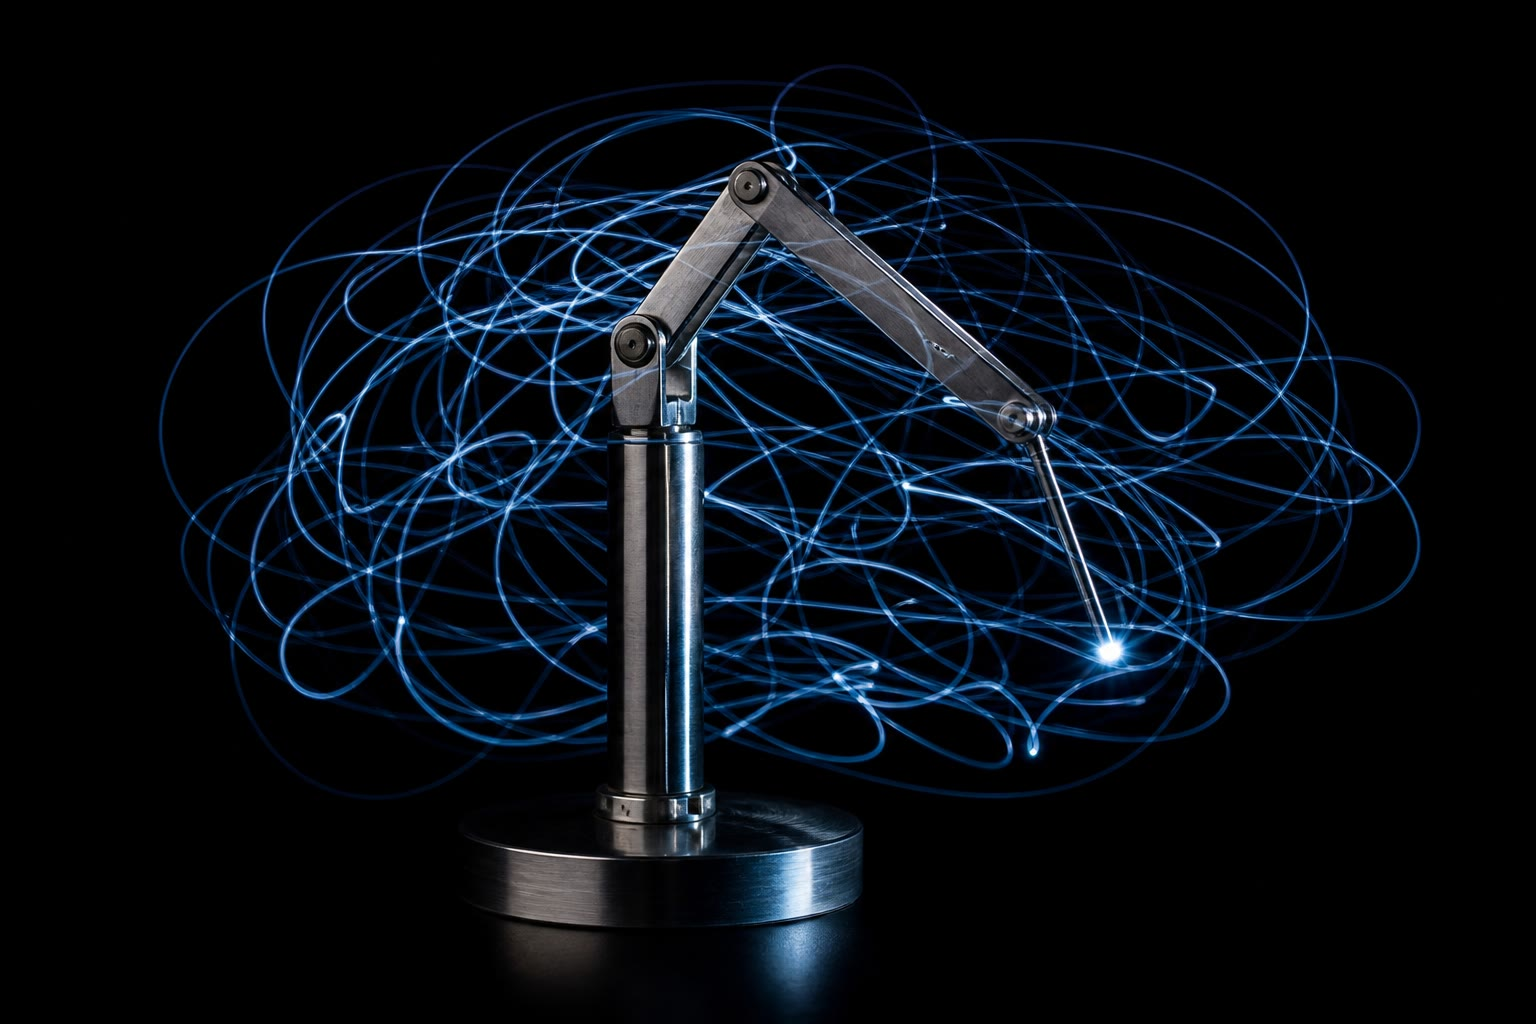
\includegraphics[width=0.58\linewidth]{images/book5/ai/b5-01-double-pendulum-trace.jpg}

{\small Bandul ganda yang jejaknya direkam dengan pajanan panjang: dua koordinat, satu \omterm{def:b3:lagrangian-mechanics:action}{Lagrangian}, dan gerak yang tak dapat diramalkan rumus mana pun untuk waktu lama --- perangkat \omterm{thm:b3:lagrangian-mechanics:euler-lagrange}{aksi terkecil} dalam bab ini menuliskan persamaannya; kekacauan membuat penyelesaiannya tetap rendah hati.}
\end{omfigure}

\section{Latihan}

\begin{exercise}[$\star$]\label{exo:b3:lagrangian-mechanics:1}
Hitunglah \omterm{def:b3:lagrangian-mechanics:coordinates}{derajat kebebasannya} dan usulkanlah \omterm{def:b3:lagrangian-mechanics:coordinates}{koordinat rampatan}: (a)
sebuah partikel di dalam mangkuk yang tetap; (b) sebuah silinder yang
menggelinding tanpa selip menuruni bidang miring yang tetap; (c) sebuah
bandul ganda yang poros atasnya meluncur pada rel mendatar; (d) sebuah
halter (dua massa, batang tegar) di ruang bebas; (e) dua manik pada satu
kawat lingkaran yang tetap. \omterm{def:b3:lagrangian-mechanics:coordinates}{Kendala} mana dalam daftar ini yang
menghubungkan kecepatan alih-alih kedudukan, dan mengapa ia toh dapat
diintegralkan menjadi \omterm{def:b3:lagrangian-mechanics:coordinates}{kendala} holonomik?
\end{exercise}

\begin{exercise}[$\star$]\label{exo:b3:lagrangian-mechanics:2}
Untuk bandul bidang (\cref{ex:b3:lagrangian-mechanics:pendulum}):
(a) periksalah dimensi $L$ dan dimensi $p_\theta =
\partial L/\partial\dot\theta$; (b) kenalilah makna fisis $p_\theta$;
(c) turunkanlah periode sudut kecilnya; (d) hitunglah \omterm{def:b3:lagrangian-mechanics:action}{aksi} $S$ satu
\omterm{prop:b3:lagrangian-mechanics:modes}{osilasi kecil} penuh beramplitudo $\theta_0$ --- lalu jelaskanlah
jawabannya sebelum menghitung (berapakah rata-rata waktu dari
$E_k - E_p$ untuk osilasi harmonik?).
\end{exercise}

\begin{exercise}[$\star$]\label{exo:b3:lagrangian-mechanics:3}
Sebuah mesin Atwood: massa $m_1$ dan $m_2$ tergantung pada tali ideal
yang melewati katrol tak bermassa. (a) Pilihlah satu koordinat dan
tuliskanlah $L$. (b) Carilah percepatannya. (c) Perlakuan Newton
memerlukan tegangan talinya --- ke manakah tegangan itu pergi? (d)
Bagaimana caranya memperoleh kembali tegangan itu setelah geraknya
diketahui?
\end{exercise}

\begin{exercise}[$\star$]\label{exo:b3:lagrangian-mechanics:4}
Sebuah partikel bebas dalam koordinat silinder: $L = \tfrac12 m(\dot r^2 +
r^2\dot\varphi^2 + \dot z^2)$. (a) Koordinat mana yang siklik, dan
apa saja momentum kekalnya? (b) Mengapa $p_r$ \emph{tidak} kekal
padahal tak ada gaya yang bekerja? (c) Tuliskanlah \omterm{thm:b3:lagrangian-mechanics:euler-lagrange}{persamaan
Euler--Lagrange} untuk $r$ dan tafsirkanlah suku $mr\dot\varphi^2$.
(d) Periksalah bahwa garis lurus yang ditempuh dengan kelajuan tetap
memenuhinya.
\end{exercise}

\begin{exercise}[$\star\star$]\label{exo:b3:lagrangian-mechanics:5}
Sebuah balok bermassa $m$ meluncur pada permukaan tanpa gesekan (bersudut
$\alpha$) sebuah baji bermassa $M$, yang sendirinya bebas meluncur di
lantai tanpa gesekan. (a) Pilihlah dua koordinat: absis baji $X$ dan
jarak balok $s$ menuruni permukaan itu; tuliskanlah $L$. (b) Koordinat
mana yang siklik, dan hukum kekekalan apa yang dinyatakannya? (c)
Carilah kedua percepatannya. (d) Periksalah limit $M \to \infty$ dan
$\alpha \to
90^\circ$.
\end{exercise}

\begin{exercise}[$\star\star$]\label{exo:b3:lagrangian-mechanics:6}
Bandul bola: sebuah bandulan pada batang sepanjang $\ell$, bebas dalam
kedua sudutnya ($\theta$ dari arah tegak ke bawah, $\varphi$
mengelilinginya). (a) Tuliskanlah $L$. (b) Kenalilah \omterm{def:b3:lagrangian-mechanics:momentum}{koordinat sikliknya}
dan $p_\varphi$ yang kekal. (c) Reduksilah gerak $\theta$ menjadi gerak
dalam potensial efektif lalu sketsalah potensial itu. (d) Untuk gerak
kerucut $\theta =
\theta_0$, perolehlah kembali hubungan bandul kerucut $\cos\theta_0 =
g/\ell\omega^2$ dari jilid Tahun 1.
\end{exercise}

\begin{exercise}[$\star\star$]\label{exo:b3:lagrangian-mechanics:7}
Sebuah bandul (massa $m$, panjang $\ell$) tergantung pada kereta
bermassa $M$ yang bebas menggelinding di rel mendatar. (a) Dengan
koordinat $X$ (kereta) dan $\theta$, tuliskanlah $L$. (b) Apa yang
kekal, dan mengapa secara fisis? (c) Linearkanlah untuk $\theta$ kecil
dan tunjukkanlah bahwa frekuensi osilasinya
$\Omega = \sqrt{(1 + m/M)\,g/\ell}$. (d) Jelaskanlah limit $M \to
\infty$ dan $M \to 0$ --- mengapa kereta yang ringan justru
\emph{menaikkan} frekuensinya?
\end{exercise}

\begin{exercise}[$\star\star$]\label{exo:b3:lagrangian-mechanics:8}
Sebuah partikel bermuatan $q$ dalam medan seragam $\vect B = B\vect e_z$,
yang digambarkan oleh $\vect A = \tfrac12\vect B\wedge\vect r$. (a)
Tuliskanlah $L$ dalam koordinat Kartesius. (b) Turunkanlah persamaan
geraknya dan periksalah bahwa persamaan itu menggambarkan lingkaran
siklotron pada $\omega_{\text{c}} = qB/m$. (c) Hitunglah momentum
konjugat $p_x$, $p_y$: apakah keduanya $m\dot x$, $m\dot y$? Apakah
keduanya kekal? (d) Tunjukkanlah bahwa $L$ yang dituliskan dalam
koordinat silinder mempunyai $\varphi$ siklik, dan kenalilah $p_\varphi$
kekal untuk lingkaran yang berpusat pada sumbunya.
\end{exercise}

\begin{exercise}[$\star\star$]\label{exo:b3:lagrangian-mechanics:9}
Untuk manik pada gelang yang berputar
(\cref{ex:b3:lagrangian-mechanics:hoop}): (a) hitunglah \omterm{prop:b3:lagrangian-mechanics:energy}{fungsi energi}
$h$ dan periksalah kekekalannya lewat persamaan gerak; (b) hitunglah
energi mekanik $E$ dan tunjukkanlah $E - h =
m\omega^2R^2\sin^2\theta$; (c) carilah daya yang diserahkan motornya
sebagai fungsi $\theta$ dan $\dot\theta$; (d) carilah frekuensi
\omterm{prop:b3:lagrangian-mechanics:modes}{osilasi kecil} di sekitar kesetimbangan miringnya ketika $\omega^2 > g/R$,
lalu tunjukkanlah bahwa frekuensi itu lenyap ketika $\omega^2 \to g/R$
--- perlambatan yang menandakan terbelahnya sumur.
\end{exercise}

\begin{exercise}[$\star\star\star$]\label{exo:b3:lagrangian-mechanics:10}
Bandul ganda yang kedua bagiannya sama ($m_1 = m_2 = m$, $\ell_1 = \ell_2 = \ell$).
(a) Tunjukkanlah bahwa untuk sudut kecil $L = \tfrac12 m\ell^2(2\dot\theta_1^2 +
2\dot\theta_1\dot\theta_2 + \dot\theta_2^2) - \tfrac12 mg\ell(2
\theta_1^2 + \theta_2^2)$. (b) Tuliskanlah kedua persamaan geraknya.
(c) Carilah frekuensi normalnya $\Omega_\pm^2 = (2 \mp \sqrt2)\,g/\ell$
dan bentuk tiap ragamnya ($\theta_2 = \pm\sqrt2\,\theta_1$). (d) Pada
amplitudo besar sistem ini menjadi contoh baku kekacauan: jelaskanlah
dalam beberapa baris apa yang meruntuhkan analisis sudut kecil, dan
mengapa tak ada hukum kekekalan yang hilang.
\end{exercise}

\begin{exercise}[$\star\star\star$]\label{exo:b3:lagrangian-mechanics:11}
\emph{Brakistokron.} Sebuah manik meluncur tanpa gesekan dari keadaan
diam di titik asal, menuruni kurva $y(x)$ ($y$ ke bawah) menuju titik
$(a, b)$. (a) Dengan kekekalan energi, tunjukkanlah bahwa waktu
turunnya adalah $T =
\int_0^a\sqrt{(1 + y'^2)/2gy}\,\dd x$ --- sebuah fungsional, dengan $x$
berperan sebagai waktu. (b) Integrannya $F(y, y')$ tidak memuat $x$
secara eksplisit: tunjukkanlah bahwa
$h = y'\,\partial F/\partial y' - F$ tetap sepanjang kurva optimalnya
(perhitungan yang sama seperti
\cref{prop:b3:lagrangian-mechanics:energy}). (c) Simpulkanlah $y(1 + y'^2) =
2r$ untuk suatu tetapan $r$, dan periksalah bahwa sikloid $x = r(\phi -
\sin\phi)$, $y = r(1 - \cos\phi)$ memenuhinya. (d) Tunjukkanlah bahwa
turunnya manik ke dasar satu lengkung memakan waktu $\pi\sqrt{r/g}$, lalu
bandingkanlah dengan peluncur lurus ke titik yang sama.
\end{exercise}

\begin{exercise}[$\star\star\star$]\label{exo:b3:lagrangian-mechanics:12}
\emph{Fermat sebagai \omterm{thm:b3:lagrangian-mechanics:euler-lagrange}{aksi terkecil}.} Cahaya dalam medium berindeks $n(y)$
menempuh perjalanan antara dua titik dalam waktu terkecil (jilid Tahun
2). (a) Tunjukkanlah bahwa waktu tempuh sepanjang $y(x)$ adalah $T = \tfrac1c\int n(y)\sqrt{1 +
y'^2}\,\dd x$. (b) Karena integrannya tidak memuat $x$ secara eksplisit,
pakailah $h$ kekal dari latihan sebelumnya untuk menunjukkan $n(y)\big/\sqrt{1 +
y'^2} = \text{const}$, dan periksalah bahwa ini adalah hukum Snellius $n\sin i =
\text{const}$ bagi sinar yang diukur dari arah tegak. (c) Di atas jalan
yang panas indeksnya bertambah terhadap ketinggian sebagai
$n(y) \approx n_0(1 + \beta y)$; tunjukkanlah bahwa sinar yang hampir
mendatar membelok dengan jari-jari kelengkungan $R \approx
1/\beta$. (d) Dengan $\beta = \qty{1.2e-5}{m^{-1}}$, dari jarak berapa
seorang pengemudi yang matanya \qty{1.2}{m} di atas jalan melihat
fatamorgana ``air'' di atasnya?
\end{exercise}

\begin{omfigure}
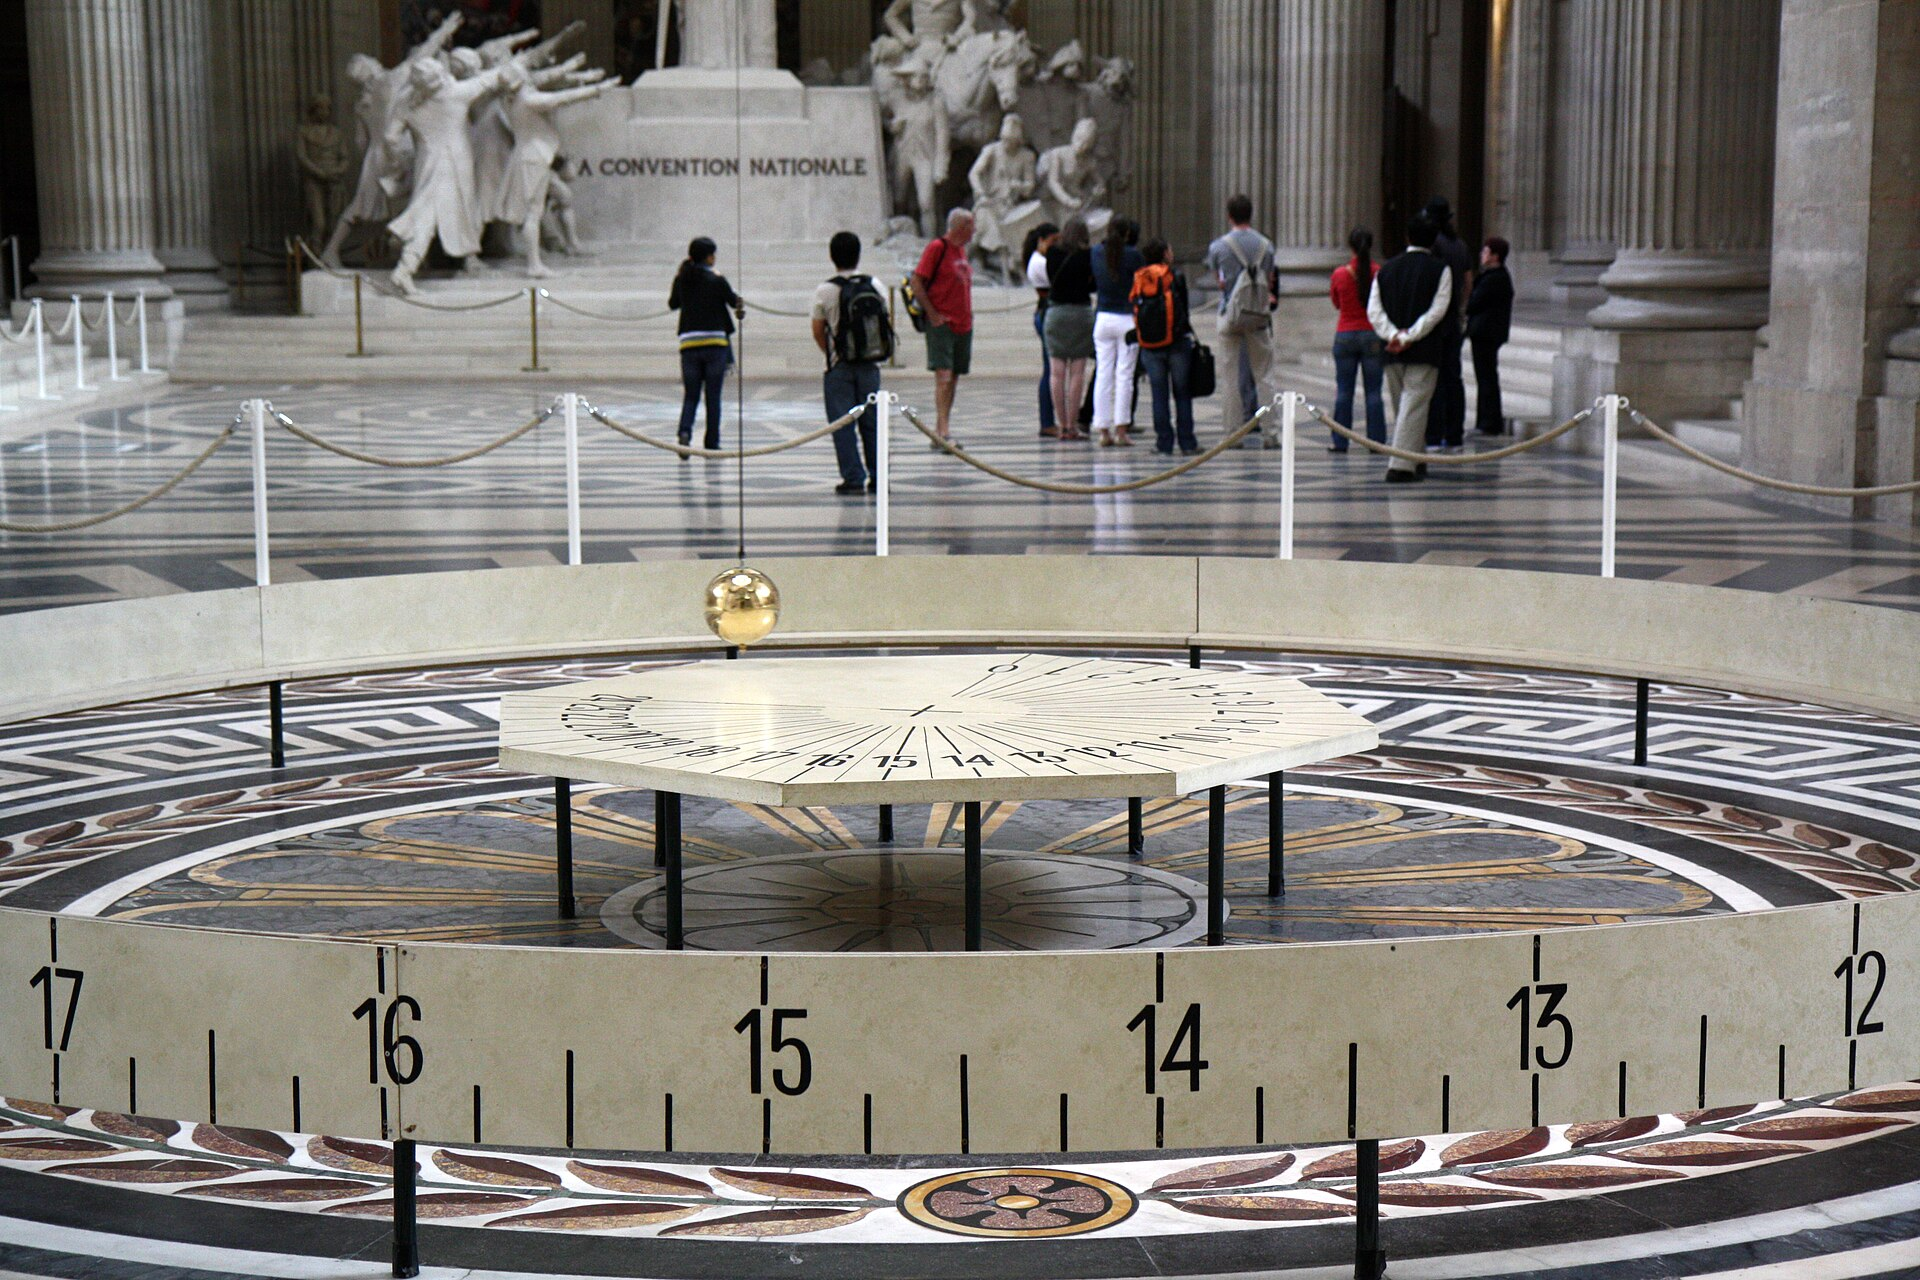
\includegraphics[width=0.6\linewidth]{images/book5/photo-foucault-pantheon.jpg}

{\small Bandul Foucault di Panteon, Paris. \omterm{def:b3:lagrangian-mechanics:coordinates}{Koordinat rampatan}, sebuah \omterm{def:b3:lagrangian-mechanics:coordinates}{kendala}, dan kerangka yang berputar perlahan: rotasi ruangannya muncul dalam persamaan geraknya --- dan pergeseran bidang ayunnya memungkinkan sebuah ruang bawah tanah mengukur putaran Bumi. Foto: Olga Khomitsevich, CC\ BY\ 2.0.}
\end{omfigure}

\section{Soal: Sapu yang berdiri terbalik}

\begin{problem}[{Soal akhir pekan --- bandul terbalik Kapitza}]\label{pb:b3:lagrangian-mechanics:1}
Sebuah bandul tegar dapat berdiri mantap \emph{di atas} porosnya jika
porosnya digoyang naik-turun cukup cepat --- penemuan yang dianalisis
Kapitza pada 1951, cukup memukau hingga tampak seperti sulap, sekaligus
asas yang dipakai medan listrik berosilasi untuk memerangkap ion tunggal.
Bandulnya kita modelkan sebagai massa titik $m$ di ujung batang tegar
tak bermassa sepanjang $\ell = \qty{40}{cm}$; $\theta$ adalah sudut dari
arah tegak \emph{ke bawah}; $g = \qty{9.81}{m/s^2}$.

\medskip\noindent\textbf{Bagian I --- Bandul tegar.}
Porosnya mula-mula ditahan tetap.
\begin{enumerate}
  \item Tuliskanlah \omterm{def:b3:lagrangian-mechanics:action}{Lagrangian} dan persamaan geraknya.
  \item Berikanlah frekuensi $f_0$ \omterm{prop:b3:lagrangian-mechanics:modes}{osilasi kecil} di sekitar $\theta =
        0$, beserta nilainya.
  \item Tunjukkanlah bahwa di sini $h = E$, lalu pakailah kekekalannya
        untuk mencari kelajuan lontar minimum bandulannya, di titik
        terbawah, yang membawanya sampai ke puncak.
  \item Linearkanlah persamaannya di dekat $\theta = \pi$ (ambil $\theta = \pi +
        \epsilon$) dan tunjukkanlah $\ddot\epsilon = +(g/\ell)\epsilon$:
        seberapa cepat kemiringan awal sebesar satu milideraja tumbuh?
        Berikanlah waktu yang diperlukannya untuk tumbuh sebesar faktor
        $e$.
  \item Sapu yang diseimbangkan di ujung jari jatuh dalam waktu sekitar
        satu sekon, namun tak pernah berdiri sendiri: nyatakanlah dalam
        satu kalimat apa yang dikatakan persamaan terlinearkan itu
        tentang kesetimbangan $\theta = \pi$.
\end{enumerate}

\medskip\noindent\textbf{Bagian II --- Menggoyang porosnya.}
Porosnya kini berosilasi tegak, dengan ketinggian $y_{\text{s}}(t) =
a\cos\Omega t$ dan $a = \qty{2.0}{cm}$, sedangkan $\Omega$ dapat diatur.
\begin{enumerate}[resume]
  \item Tuliskanlah koordinat bandulannya dan tunjukkanlah
        $\vect v^{\,2} = \ell^2\dot\theta^2 -
        2a\Omega\ell\sin(\Omega t)\sin\theta\,\dot\theta +
        a^2\Omega^2\sin^2\Omega t$.
  \item Tunjukkanlah bahwa dua \omterm{def:b3:lagrangian-mechanics:action}{Lagrangian} yang berbeda sebesar suatu
        turunan waktu total $\dd F(q,t)/\dd t$ memberikan \omterm{thm:b3:lagrangian-mechanics:euler-lagrange}{persamaan
        Euler--Lagrange} yang sama.
  \item Dengan kebebasan itu, sederhanakanlah \omterm{def:b3:lagrangian-mechanics:action}{Lagrangiannya} menjadi $L = \tfrac12 m
        \ell^2\dot\theta^2 - ma\Omega^2\ell\cos(\Omega t)\cos\theta +
        mg\ell\cos\theta$. (Petunjuk: $\sin(\Omega t)\sin\theta\,\dot\theta$
        bergabung dengan suku $\cos(\Omega t)\cos\theta$ menjadi sebuah
        turunan total; suku yang hanya memuat $t$ boleh dibuang.)
  \item Turunkanlah persamaan geraknya
        \[
        \ddot\theta = -\frac{g}{\ell}\sin\theta
         + \frac{a\Omega^2}{\ell}\cos(\Omega t)\sin\theta .
        \]
        Tafsirkanlah suku keduanya sebagai berat yang digantikan oleh $g +
        \ddot y_{\text{s}}$: bandulnya hidup di dalam lift.
  \item Apakah \omterm{prop:b3:lagrangian-mechanics:energy}{fungsi energi} $h$ masih kekal sekarang? Apakah energinya
        kekal? Apa yang memompa energi masuk dan keluar?
  \item Dalam rezim Kapitza $a \ll \ell$ dan $\Omega \gg \omega_0 =
        \sqrt{g/\ell}$: periksalah keduanya untuk $a = \qty{2}{cm}$, $\ell =
        \qty{40}{cm}$, $\Omega/2\pi = \qty{40}{Hz}$, lalu jelaskanlah
        secara fisis mengapa bandulannya kemudian tak dapat mengikuti
        goyangan itu.
\end{enumerate}

\medskip\noindent\textbf{Bagian III --- Memisahkan yang cepat dari yang lambat.}
Carilah geraknya dalam bentuk $\theta(t) = \Theta(t) + \xi(t)$: hanyutan
lambat $\Theta$ ditambah riak kecil $\xi$ pada frekuensi goyangannya.
\begin{enumerate}[resume]
  \item Dengan mempertahankan hanya suku terbesar di tiap ruas,
        tunjukkanlah bahwa riaknya memenuhi
        $\ddot\xi \approx +(a\Omega^2/\ell)\cos(\Omega t)
        \sin\Theta$, dengan $\Theta$ dibekukan pada skala waktu goyangan.
  \item Simpulkanlah $\xi(t) = -(a/\ell)\cos(\Omega t)\sin\Theta$, lalu
        periksalah bahwa amplitudonya kecil, berorde $a/\ell$.
  \item Jabarkanlah $\sin\theta = \sin(\Theta + \xi)$ sampai orde
        pertama dalam $\xi$ lalu masukkanlah ke persamaan geraknya.
  \item Rata-ratakanlah atas satu periode goyangan, dengan $\Theta$
        ditahan tetap: dengan $\langle\cos\Omega t\rangle = 0$ dan
        $\langle\cos^2\Omega t\rangle = \tfrac12$, tunjukkanlah
        \[
        \ddot\Theta = -\frac{g}{\ell}\sin\Theta
         - \frac{a^2\Omega^2}{2\ell^2}\sin\Theta\cos\Theta .
        \]
  \item Tunjukkanlah bahwa ini adalah gerak dalam potensial efektif
        \[
        U_{\text{eff}}(\Theta) = mg\ell\Big({-\cos\Theta}
         + \frac{a^2\Omega^2}{4g\ell}\sin^2\Theta\Big) .
        \]
  \item Bandingkanlah dengan manik pada gelang yang berputar
        (\cref{ex:b3:lagrangian-mechanics:hoop}): matematikanya sama,
        tanda suku barunya berlawanan --- apa yang dilakukan goyangan
        itu terhadap kesetimbangan \emph{terbawah}, yang tidak dilakukan
        rotasi tadi?
  \item Sketsalah $U_{\text{eff}}$ untuk goyangan lambat dan untuk
        goyangan cepat, lalu uraikanlah setiap kesetimbangan beserta
        kemantapannya pada masing-masing kasus.
\end{enumerate}

\medskip\noindent\textbf{Bagian IV --- Sapunya berdiri.}
\begin{enumerate}[resume]
  \item Dengan menjabarkan $U_{\text{eff}}$ di dekat $\Theta = \pi$,
        tunjukkanlah bahwa kedudukan terbaliknya mantap tepat ketika
        \[
        a^2\Omega^2 > 2g\ell .
        \]
  \item Hitunglah frekuensi goyangan kritis $f_{\text{c}} =
        \Omega_{\text{c}}/2\pi$ bagi bandul kita, serta kelajuan puncak
        porosnya $a\Omega_{\text{c}}$ dan percepatan
        $a\Omega_{\text{c}}^2$ (dalam satuan $g$) yang dituntutnya.
  \item Pada $\Omega = 2\Omega_{\text{c}}$, carilah frekuensi ayunan
        lambat bandul yang berdiri itu di sekitar $\Theta = \pi$,
        beserta nilainya; periksalah bahwa frekuensi itu memang lambat
        dibandingkan goyangannya.
  \item Masih pada $\Omega = 2\Omega_{\text{c}}$, berapakah amplitudo
        riak $\xi$ ketika $\Theta$ sedikit menyimpang dari $\pi$, dalam
        derajat, untuk $a/\ell = 0.05$? Akankah sebuah foto membongkar
        sulapnya?
  \item Seberapa jauh dari arah tegak sapunya boleh miring dan masih
        kembali? Tunjukkanlah bahwa sumur berdirinya membentang sepanjang $|\Theta - \pi| <
        \arccos(2g\ell/a^2\Omega^2)$, lalu hitunglah nilainya pada $\Omega =
        2\Omega_{\text{c}}$.
  \item Seorang pemain sulap yang menyeimbangkan sapu di ujung jari yang
        diam juga menjaganya tetap tegak --- lewat mekanisme yang sama
        sekali berbeda yang mana? Sebutkanlah ciri bandul Kapitza yang
        tidak memerlukan umpan balik.
  \item Ringkaslah hasil bernama itu: poros yang digoyang dengan
        amplitudo \qty{2}{cm} pada \qty{45}{Hz} --- dua kali frekuensi
        kritisnya --- menahan bandul sepanjang \qty{40}{cm} dalam
        keadaan terbalik, di dalam sumur yang mencapai sekitar
        $75^\circ$ dari arah tegak, sambil berayun lembut pada sekitar
        \qty{1.4}{Hz}. Di bagian fisika manakah perangkap rata-rata yang
        sama dipakai untuk menahan satu partikel bermuatan?
\end{enumerate}
\end{problem}
